\section{Black Holes \& Star Formation} \label{Sec: Active Galactic Nuclei}
Over 100 years ago, Einstein's theory of General Relativity \citep{einstein_feldgleichungen_1915} predicted black holes to exist. \cite{webster_cygnus_1972} discovered the first black hole with X-ray observations of binary stellar-mass-sized black holes. However, black holes have existed since at least the beginning of the \gls{eor} \citep{barkana_beginning_2001}.

\gls{agn} are actively accreting supermassive black holes (SMBH) whereby massive quantities of interstellar material power their growth \citep{hopkins_cosmological_2008, han_evolution_2012, toba_9_2013, brown_infrared_2019}. In the local universe, it is widely accepted that most, if not all galaxies, host a SMBH at their centre \citep{gruppioni_modelling_2011, han_evolution_2012, brown_infrared_2019}. Not all central SMBHs are active, however, as evidenced by \cite{ghez_high_1998} (see also \citealp{balick_intense_1974, genzel_stellar_2000}) who inferred the existence of a $\approx 4 \times 10^{6}\ M_{\odot}$ SMBH, named \textit{Sagittarius A$^*$}, at the centre of our own \textit{Milky Way}. The \cite{event_horizon_telescope_collaboration_first_2022} team later imaged \textit{Sagittarius A$^*$}. \cite{gruppioni_modelling_2011} finds evidence that most, if not all galaxies have at least experienced the influence of an \gls{agn} in their past. 

\subsection{AGN Classification}
The unified AGN model posits two distinct types of AGN \citep{urry_unified_1995, toba_9_2013}. Type 1 AGNs are characterized by broad emission lines in their spectra (due to high-velocity material) and provide an unobstructed view along the direct line of sight to their centres. Conversely, Type 2 AGNs exhibit only narrow emission lines associated with an obscured line of sight to the centre. In these cases, direct observation of the broad-line region is blocked or heavily absorbed by intervening material such as the dusty torus. As a result, early research often relied on X-ray \citep{miyaji_detailed_2015} and UV \citep{paltani_vimos_2007} wavelengths, but these regimes tend to omit many Type 2 AGN galaxies from their analyses. The dusty torus surrounding the black hole absorbs most of the outgoing optical, UV, and X-ray radiation, re-emitting it primarily in the \gls{ir} spectrum \citep{fu_decomposing_2010, wu_mid-infrared_2011, assef_mid-ir-_2011, han_evolution_2012, toba_9_2013, brown_infrared_2019, symeonidis_agn_2021}, underscoring the importance of IR observations in addition to other wavelengths. Some research questions the unified AGN model and argues that the phenomenon of AGN obscuration is significantly more complex than simple viewing angles suggest. \cite{han_evolution_2012} concluded that the obscuration caused by the dusty torus must evolve, and \cite{brown_infrared_2019} agrees, observing that the line of sight to AGNs does not determine the resulting AGN type.

\begin{figure}[t!]
    \centering
    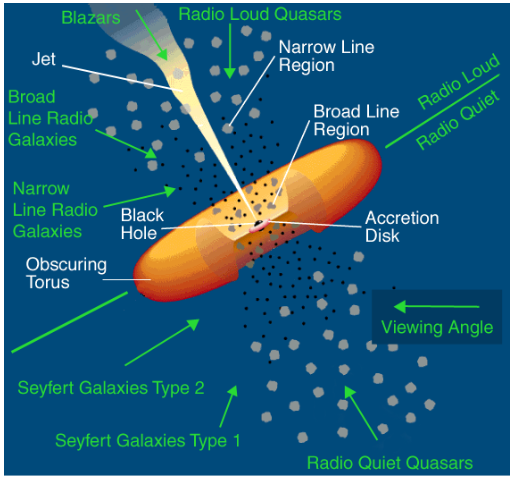
\includegraphics[width=0.9\linewidth]{Figures/agn_diagram_cc.png}
    \caption{Diagram of an AGN. Viewing angles differentiate AGN types: Blazars directly observe the jet; type 2 the thick dusty torus; and type 1 in between (Credit: \citealp{urry_unified_1995}, reproduced with © permission.).}
    \label{Fig: AGN Diagram}
\end{figure}

The ambiguity surrounding the existence of various AGN types can be confusing; however, sight lines are crucial in our observations of AGN, particularly those dust-enshrouded and obscured. The classification of AGN remains a contentious issue \citep{padovani_active_2017}, with \cite{hickox_obscured_2018} referring to it as a ``menagerie." \Cref{Fig: AGN Diagram} presents a typical AGN and the general classification when viewed from various inclination angles \citep{urry_unified_1995}. When observed from a ``top-down" perspective, powerful jets emit vast quantities of radio waves and gamma-ray radiation from a highly magnetized rotating SMBH \citep{blandford_relativistic_2019}. These AGNs are classified as ``Blazars" when the jets are directed toward the observer. Both \cite{peterson_introduction_1997} and \cite{tadhunter_introduction_2008} highlight the vast array of AGN types, which can often be challenging to grasp. Fortunately, our understanding of how AGNs form and evolve is gradually improving.

